A equação de capacidade para ruído de canal aditivo, branco e gaussiano de Shannon é:

\begin{equation}
    C = B \, log_2\left(1+ SNR\right)
\end{equation}

Onde:
\begin{itemize}
    \item $C$ é a capacidade do sinal em [bits/s];
    \item $B$ é a largura de banda do canal em [Hz];
    \item e $SNR$ é a relação sinal-ruído [adimensional];
\end{itemize}

\begin{figure}[H]
\begin{center}
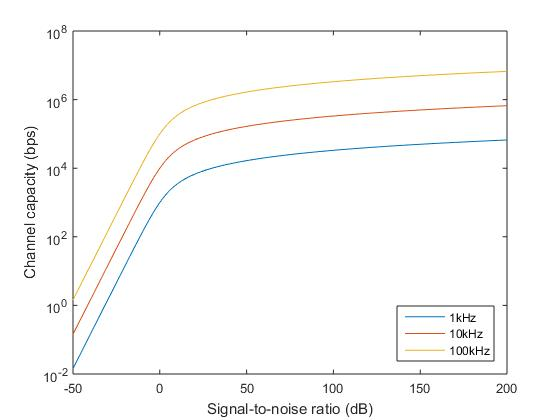
\includegraphics[width=11cm]{untitled.jpg}
\caption{Gráfico de capacidade do canal para vários valores de banda e SNR. Fonte: própria.}
\label{fig:1} 
\end{center}
\end{figure}

Devido ao comportamento logarítmico, ao variar a SNR com a banda fixa, observa-se que para valores negativos de SNR (dB) a capacidade possui uma curva de crescimento bastante agudo, porém quando chega a altos valores de SNR a taxa de crescimento da capacidade se reduz. Com o aumento da banda do canal a curva é deslocada para valores maiores, porém com a mesma tendência de crescimento.